
\documentclass{article}
\usepackage[a4paper, margin={3cm, 1.5cm}]{geometry} % Document format
\usepackage[utf8]{inputenc} % Unicode symbols
\usepackage[T1]{fontenc}
\usepackage{graphicx} % Required for inserting images
\usepackage[ngerman]{babel}
\usepackage{amsmath}
\usepackage{amssymb}
\usepackage{afterpage}
\usepackage{hyperref}

% Bibliography
\usepackage{csquotes}
\usepackage[
backend=biber,
style=alphabetic,
sorting=ynt
]{biblatex}
\addbibresource{bib/all.bib}    % Where the citing information is stored

\title{
    RC-Hochpassfilter \\
    Laborbericht Schwerpunktfach Physik
}
\author{Hanna Shubina, Lars Hösli}
\date{Februar 2024}


\begin{document}

\maketitle

%------------- Introduction -------------%
\section{Problemstellung}

RC-Glieder (engl. Resistor-Capacitor) bezeichnet eine bestimmte Art von Vier-Pol-Schaltungen, die aus einem Widerstand und einem Kondensator bestehen. Der Kondensator besitzt Frequenzabhängig einen unterschiedlischen elektrischen Widerstand beziehungsweise Scheinwiderstand. Diese Eigenschaft kann benutzt werden, damit nur gewisse Frequenzen durch den Kondensator gelassen werden können. Der Widerstand bietet dann einen alternativen Weg für den Strom, den der Strom für die übrigen Frequenzen nehmen kann.

\subsection{RC-Hochpassfilter}
Auf diese Weise kann ein gewisses Spektrum von Signalen gefiltert werden. Wird der Verbraucher nach dem Kondensator geschaltet und der Widerstand parallel zum Verbraucher, werden die kurzwelligen Signale durch den Kondensator und den Verbraucher gelassen während der Widerstand die langwelligen Signale direkt zum anderen Pol der Spannungsquelle leitet.
Es entsteht ein Hochpassfilter, der die Signale mit einer tiefen Frequenz wegschneidet.

\subsection{Grenzfrequenz}
Welche Signale durchgelassen und welche geschwächt oder geblockt werden, kann mithilfe der Grenzfrequenz $f_G$ beschrieben werden. Diese ist gegeben durch
\[
    f_G = \frac{1}{2\pi RC}
\]
Wobei $R$ der verwendete Widerstand und $C$ die Kapazität des Kondensators ist. Alle Frequenzen, die unter dieser Grenze liegen, können den Kondensator annäherungsweise ungehindert passieren, während die darüber geschwächt oder blockiert werden.


%------------- Fragestellung -------------%
\section{Fragestellung}
\begin{enumerate}
    \item Was ist ein gutes Verhältnis von Kondensatorkapazität und Widerstand für einen Hochpassfilter?
    \item Wie verhält sich das Signal qualitativ, wenn das Kondensator-Resistor Verhältnis nicht stimmt?
    \begin{itemize}
        \item Wie gut entspricht empirisch erhobene Werte den Erwartungswerten?
    \end{itemize}
\end{enumerate}

% TODO: Hypothese

%------------- Method -------------%
\section{Versuchbeschreibung}
Das Gerät, dass das ursprüngliche elektrische Signal generierte war eine sogennante \emph{Sound Maschine} von \emph{Kosmos} \cite{sound_machine_experimentierkasten_kosmos}.
Diese wurde dazu verwendet, eine stetige Wechselstromspannung zu generieren. Dafür wurde die Frequenz der \emph{Orgel} auf $\frac{1000}{8}Hz$ gestellt und die Amplitude auf maximal $\approx 250mV$, wie aus den erzeugten Diagrammen ausgelesen werden kann. Die erhobene Kurve des Inputsignals ähnelte einem Rechtecksignal mit einem seriegeschalteten Induktor \ref{img:c0_r47}.

Für das RC-Glied wurde mithilfe eines Arduino-Steckbrettes und Kabeln ein typischer Schaltkreis für einen Hochpassfilter (\ref{fig:circuit}) gemacht. Der Aufbau kann in Abbildung \ref{img:setup_close} betrachtet werden. Das RC-Glied wurde zwischen dem \emph{Sound Machine} \cite{sound_machine_experimentierkasten_kosmos} und dem \emph{Lautsprecher} eingebaut.

Damit das Inputsignal aus dem Audioanschluss der \emph{Sound Machine} verändert werden konnte bevor es in den \emph{Lautsprecher} geleitet wurde, wurde das Audiokabel aufgeschnitten und an die freigegebenen Kontakte wurden Drähte angelötet.

Von einem handelsübliches Oszilloskop wurde einerseits die Spannung des Inputsignals, das direkt aus dem Audiooutput herauskam, gemessen, wie auch das transformierte Signal, als die Spannung, die den Lautsprecher erreicht \ref{img:setup_close}.

\begin{figure}[htp]
    \minipage{0.49\textwidth}
        \centering
        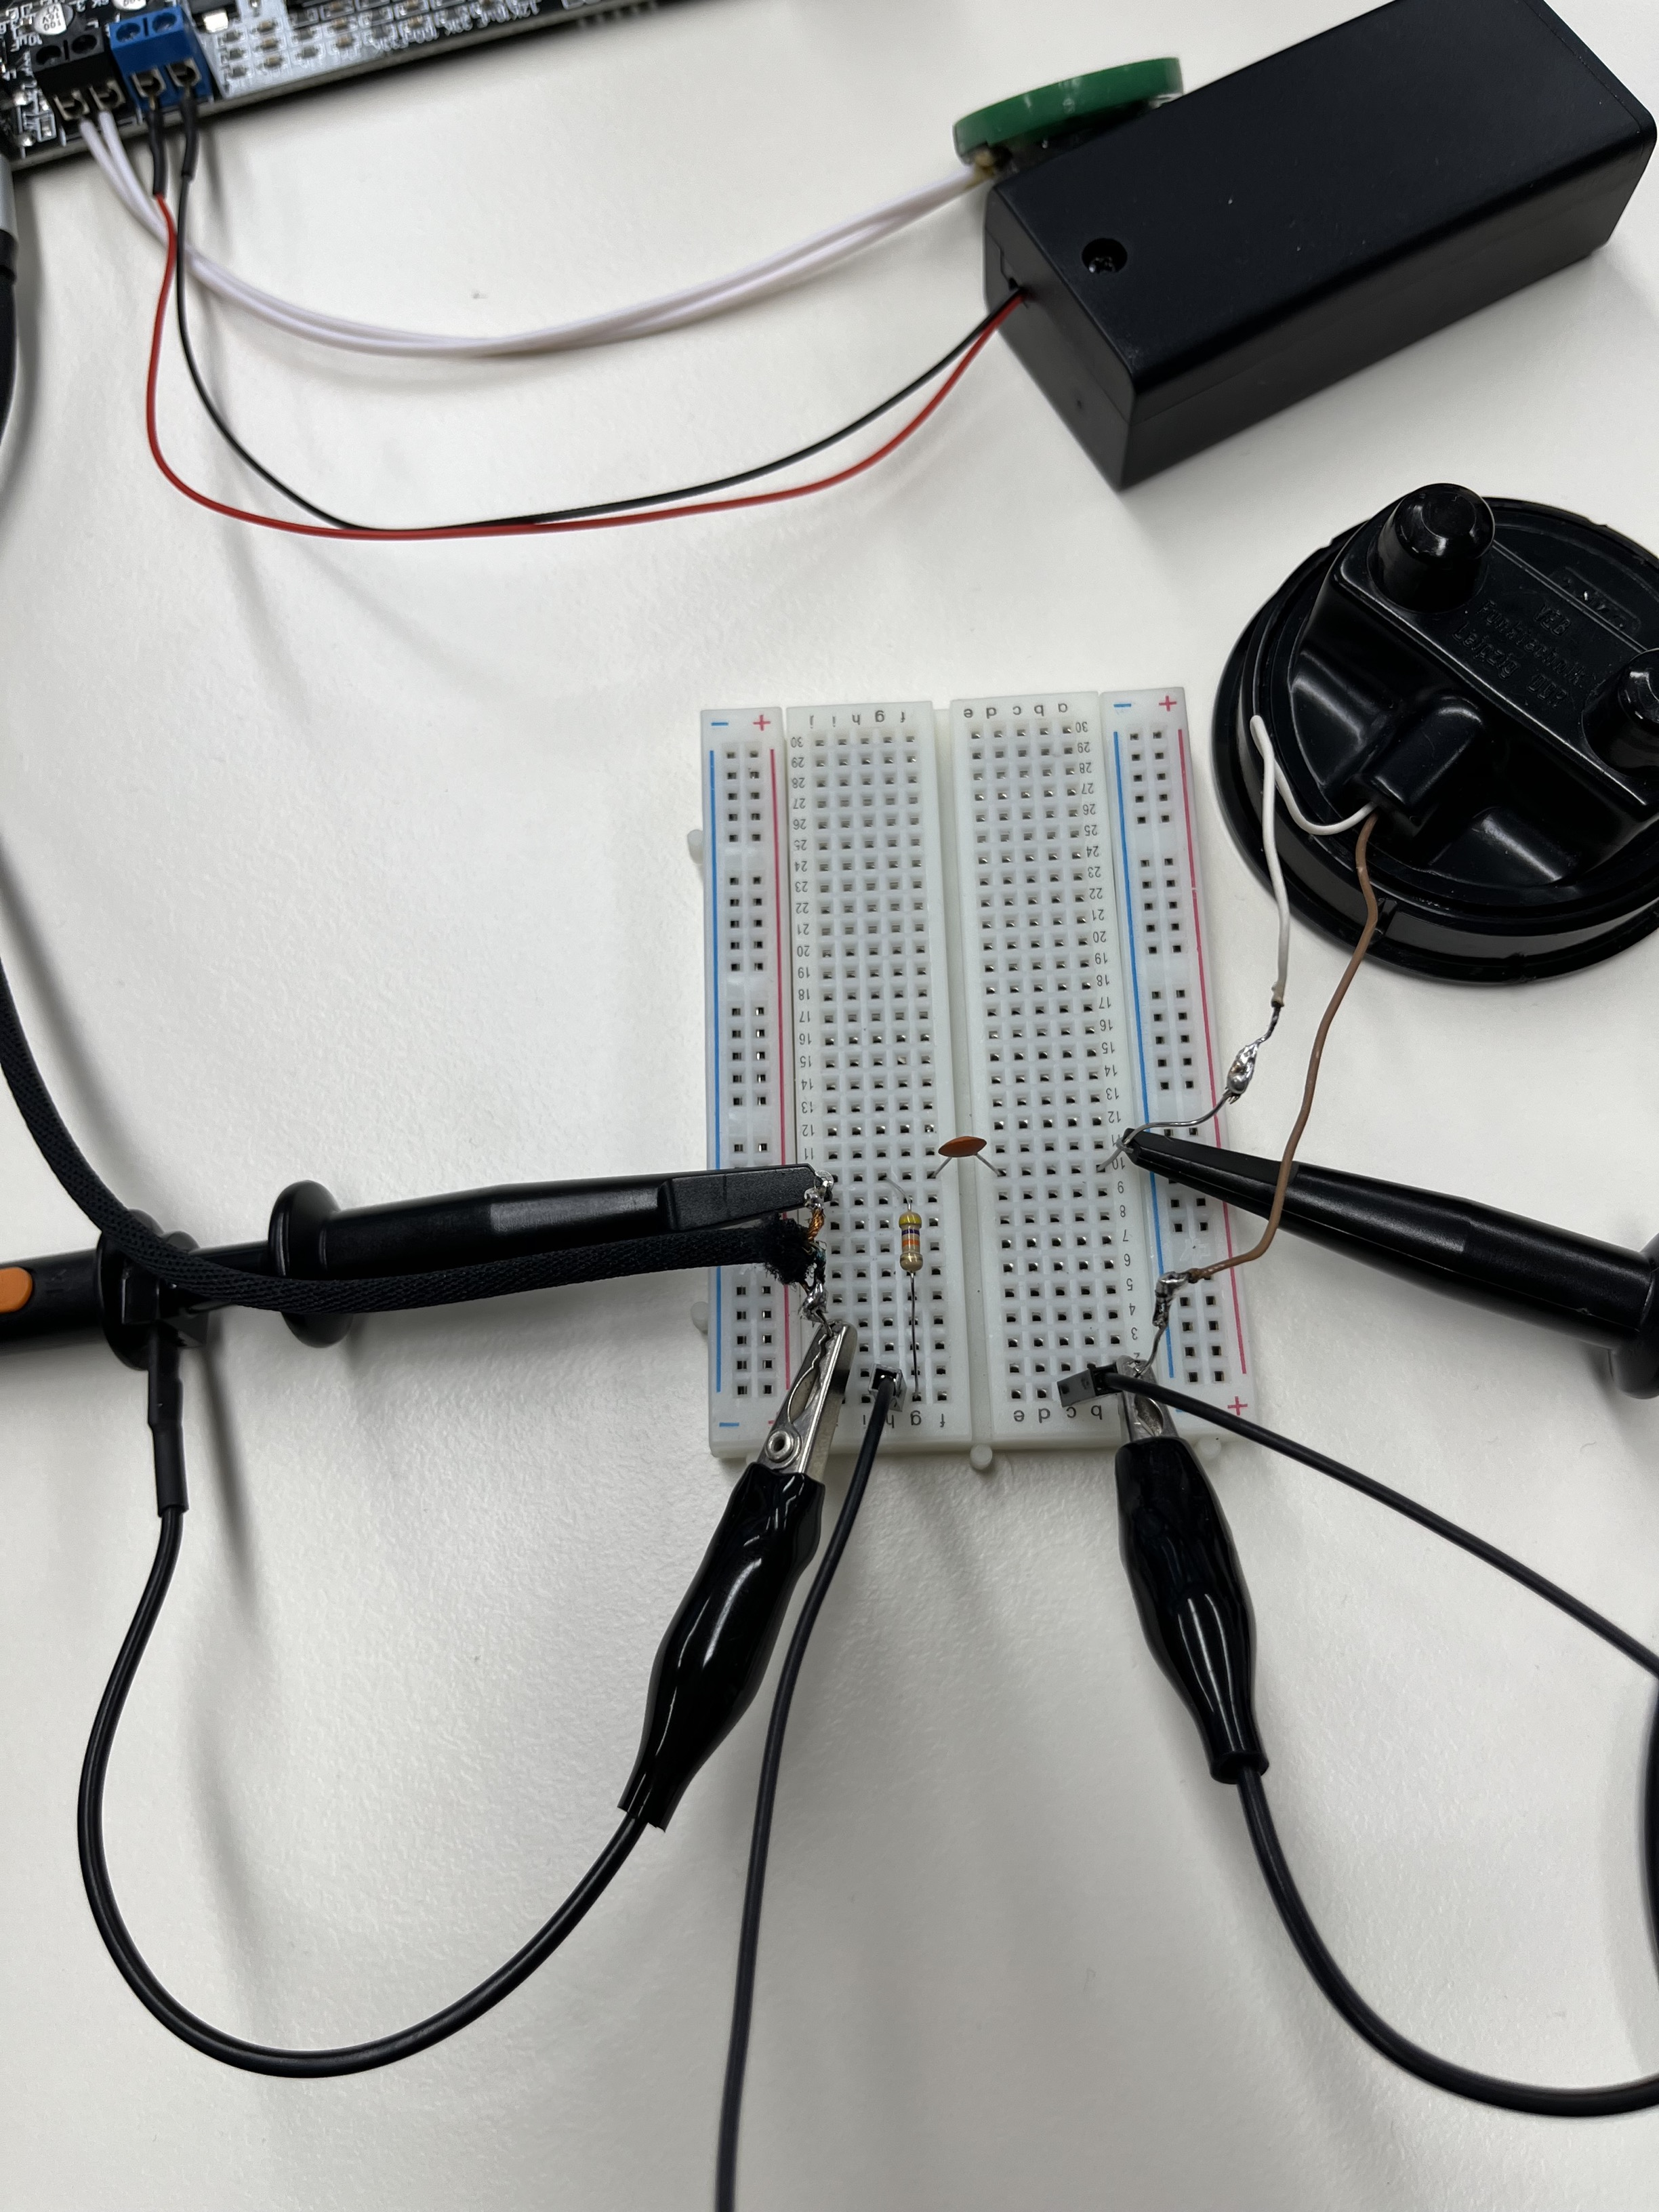
\includegraphics[width=\linewidth]{figures/setup_close.png}
        \caption{Steckbrett mit Verkabelung. Oben links im Bild befindet sich die \emph{Sound Machine}, von welcher das Inputsignal kommt. Dies entspricht der gelben Kurve in den Messungen (\ref{img:c33e0_r47}, \ref{fig:showcase_c33e1_r47} ..)}
        \label{img:setup_close}
    \endminipage\hfill
    \minipage{0.49\textwidth}
        \centering
        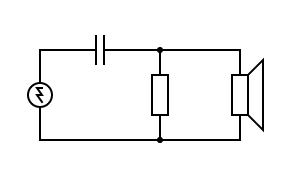
\includegraphics[width=\linewidth]{figures/circuit.png}
        \caption{Schaltkreis des Hochpassfilters. Das Schaltsymbol am ganz links steht für den Oszillator, das rechts für den Lautsprecher. Dazwischen ist die typische RC-Schaltung für Hochpassfilter mit Kondensator und Widerstand. Die Beträge der Kapazität und Widerstand wurden jeweilst variiert.}
        \label{fig:circuit}
    \endminipage\hfill
\end{figure}

%------------- Durchführung -------------%
\section{Durchführung}

Die effektive elektrische Widerstand der verwendeten Widerstände wurden mit einem handelsüblichen Multimeter nachgemessen. Dabei wurde bei dem $180k\Omega$ Widerstand ein Wert von $190k\Omega$ gemessen. Der gemessene Widerstand wurde verwendet für die Auswertung. Beim $47k\Omega$ Widerstand wurden Werte von $47k\Omega \pm 1k\Omega$ gemessen, folglich wurde der angegebene Wert verwendet, auf Ganzzahlen gerundet.

Für die zwei Widerstände ($47k\Omega$ und $190k\Omega$) wurde jeweils jeder der sieben verwendeten Kondensatoren eingesetzt (\ref{capacitors}), an der gleichen Stelle wie der Kondensator im Schaltplan \ref{fig:circuit}.

Die auf dem Oszilloskop angezeigten Werte wurden per Screenshot-Funktion des Oszilloskopes auf einen USB-Stick gespeichert und ausgewerted. 

Folgende äussere Bedingungen waren gegeben beziehungsweise wurde festgelegt:
\begin{itemize}
    \item Widerstand: 190 kOm
    \item Frequenz: 166.7 Hz
    \item Kondensatoren: Siehe Tabelle \ref{tab:capacitors}
\end{itemize}

\begin{table}[ht]
    \centering
    \begin{tabular}{c|c|p{2.5cm}}
         Code       & \multicolumn{2}{c}{Kapazität} \\
         \hline\hline
                    & SI-Untereinheiten & Wissenschaftliche Schreibweise \\
         \hline
         $33, 330$  & $33p F$   & $33 \cdot 10^{-12} F$ \\
         $68, 680$  & $68p F$   & $68 \cdot 10^{-12} F$ \\
         $331$      & $330p F$  & $33 \cdot 10^{-11} F$ \\
         $681$      & $680p F$  & $68 \cdot 10^{-11} F$ \\
         $332$      & $3300p F$ & $33 \cdot 10^{-10} F$ \\
         $682$      & $6800p F$ & $68 \cdot 10^{-10} F$ \\
         $333$      & $33n F$   & $33 \cdot 10^{-9} F$ \\
         $683$      & $68n F$   & $68 \cdot 10^{-9} F$ \\
    \end{tabular}
    \caption{Liste der verwendeten Kondensatoren}
    \label{tab:capacitors}
\end{table}


%------------- Auswertung -------------%
\section{Auswertung}


\subsection{Erwartete Grenzwerte}

Mit den gegebenen Werten und der Formel für die Grenzfrequenz kann der Grenzwert für die Kondensatorkapazität ausgerechnet werden, welcher mit dem Wert des Widerstandes aussagt, ob die Kurve sich ändern sollte durch das RC-Glied oder nicht.
\\

Dies kann erreicht werden durch eine einfache Umformung der Formel der Grenzfequenz.
\begin{align}
    f_G &= \frac{1}{2\pi RC}    \\
    C   &= \frac{1}{2\pi R f_G}
\end{align}
Für $R = 47k\Omega$ und $f_G = 166.7Hz$:
\begin{align}
    C &= \frac{1}{2\pi \cdot 47 \cdot 10^3 \cdot 166.7} \\
      &= 20'314pF
\end{align}
Und für $R = 190k\Omega$ bei gleicher Frequenz:
\begin{align}
    C = &= \frac{1}{2\pi \cdot 190 \cdot 10^3 \cdot 166.7}  \\
        &= 5'025pF
\end{align}


\subsection{Berechnung der Fläche zwischen den Kurven (Differenz der Integrale)}

Die quantitative Abweichung zwischen dem Inputsignal und dem gefilterten Signal wurde ebenfalls verglichen in den folgenden vier Graphen. Dazu wurde der Integral ausgerechnet und vom Signal vor und nach dem RC-Glied.

\begin{itemize}
    \item[$47k\Omega$] Die Integrale der Kurven des grössten ($68'000pF$) und kleinsten ($33pF$) Kondensators wurde verglichen bei einem Widerstand von $47k\Omega$.
    \item[$190k\Omega$] Dieselben Werte wurden auch für einen Widerstand von $190k\Omega$ und die Kondensatoren mit $33pF$ und $68'000pF$ erfasst.
\end{itemize}

Die erhaltenen Werte können in der Tabelle \ref{tab:integrals} ausgelesen werden.

\begin{table}[ht]
    \centering
    \begin{tabular}{ c|c c }
                    & $47.3k\Omega$ & $190k\Omega$ \\
        \hline
        $33pF$      & 451,1 & 448,3 \\
        $68'000pF$  & 198,3 & 362,3
    \end{tabular}
    \caption{Fläche zwischen den Kurven der jeweiligen Widerstände und Kondensatoren}
    \label{tab:integrals}
\end{table}

\subsubsection{Ablesen von Diagrampunkten aus einer Grafik}

Für die automatisierte Auswertung der ausgewählten Kurven wurde die Webseite \emph{automeris.io} verwendet (\cite{automeris_webplotdigitizer_webpage}). Dort kann der Benutzer ein Bild hochladen, den Bereich auswählen, aus dem er die Daten lesen möchte, und die Koordinaten (im kartesischen System) sowie die entsprechenden Achsen festlegen. 
Das Intervall auf der x-Achse betrug 2ms und die y-Achse 100mV.

Mit Hilfe der Funktion zum Lesen der Daten nach Farben und der Einstellung bestimmter anderer Daten, wie z. B. der Auflösung des Diagramms, der Genauigkeit usw., war es dann möglich, ein grafisches Bild und eine Liste der Koordinaten im .odt-Dokumentformat zu erhalten.
Dieses Verfahren wurde jeweils für beide Kurven (blau und gelb) durchgeführt.

\subsubsection{Datenanalyse} 

Die Daten wurden mithilfe von Excel weiter analysiert.

Zunächst rundeten wir die Datenpunkte aus beiden Diagrammen (gelb und blau) mit der Funktion ROUNDDOWN auf 3 Dezimalstellen.
Das Problem in dieser Phase bestand darin, dass die verschiedenen Diagramme aufgrund der unterschiedlichen Auflösungswerte, die zur Extraktion der Punkte aus dem Bild verwendet wurden, unterschiedliche Werte für das X-Intervall aufwiesen (Phasenverschiebung). Aus diesem Grund wurde jeweils eine Periode bestimmt (Maximum zu Maximum), und die y-Werte dazwischen verwendet. Dies wurde erreicht mit der Funktion LOOKUP, deren Kern darin bestand, die gemeinsamen Werte von X für beide Diagramme zu finden und die entsprechenden Werte für Y auszuschreiben.

Da nun eine gemeinsame X-Achse und zwei unterschiedliche Y-Achsen-Datensätze (\ref{img:excel_example}) vorhanden waren, konnte ein Diagramm erstellt und mit dem Originalbild verglichen werden.

\subsubsection{Berechnen der Fläche} 

Es sollte beachtet werden, dass alle nachfolgenden Berechnungen die Fläche zwischen den Kurven für eine Periode darstellen.

Die entscheidenden Schritte zur Berechnung der Fläche zwischen den Diagrammen waren wie folgt.

\begin{enumerate}
    \item Ermittlung des Moduls der Differenz in Y mit Hilfe der ABS-Funktion und einfacher Subtraktion
    \item Auswahl der Periode T des Diagramms: Anhand des Diagramms selbst konnten wir grob erkennen, wo die Periode beginnen und enden würde, aber um einen genaueren Bereich zu wählen, konzentrierten wir uns auf die Werte von y und wann sie gegen Null gehen.
    \item Die Berechnung der Fläche mit der Trapezmethode ist eine Methode zur Annäherung an den Wert eines gegebenen Integrals, indem die Fläche unter dem Graphen einer Funktion mit einem Trapez angepasst und dessen Fläche berechnet wird.
\end{enumerate}

In Excel wurde dies mit der Funktion SUMPRODUCT erreicht (\ref{img:excel_example}).

\begin{figure}[ht]
    \centering
    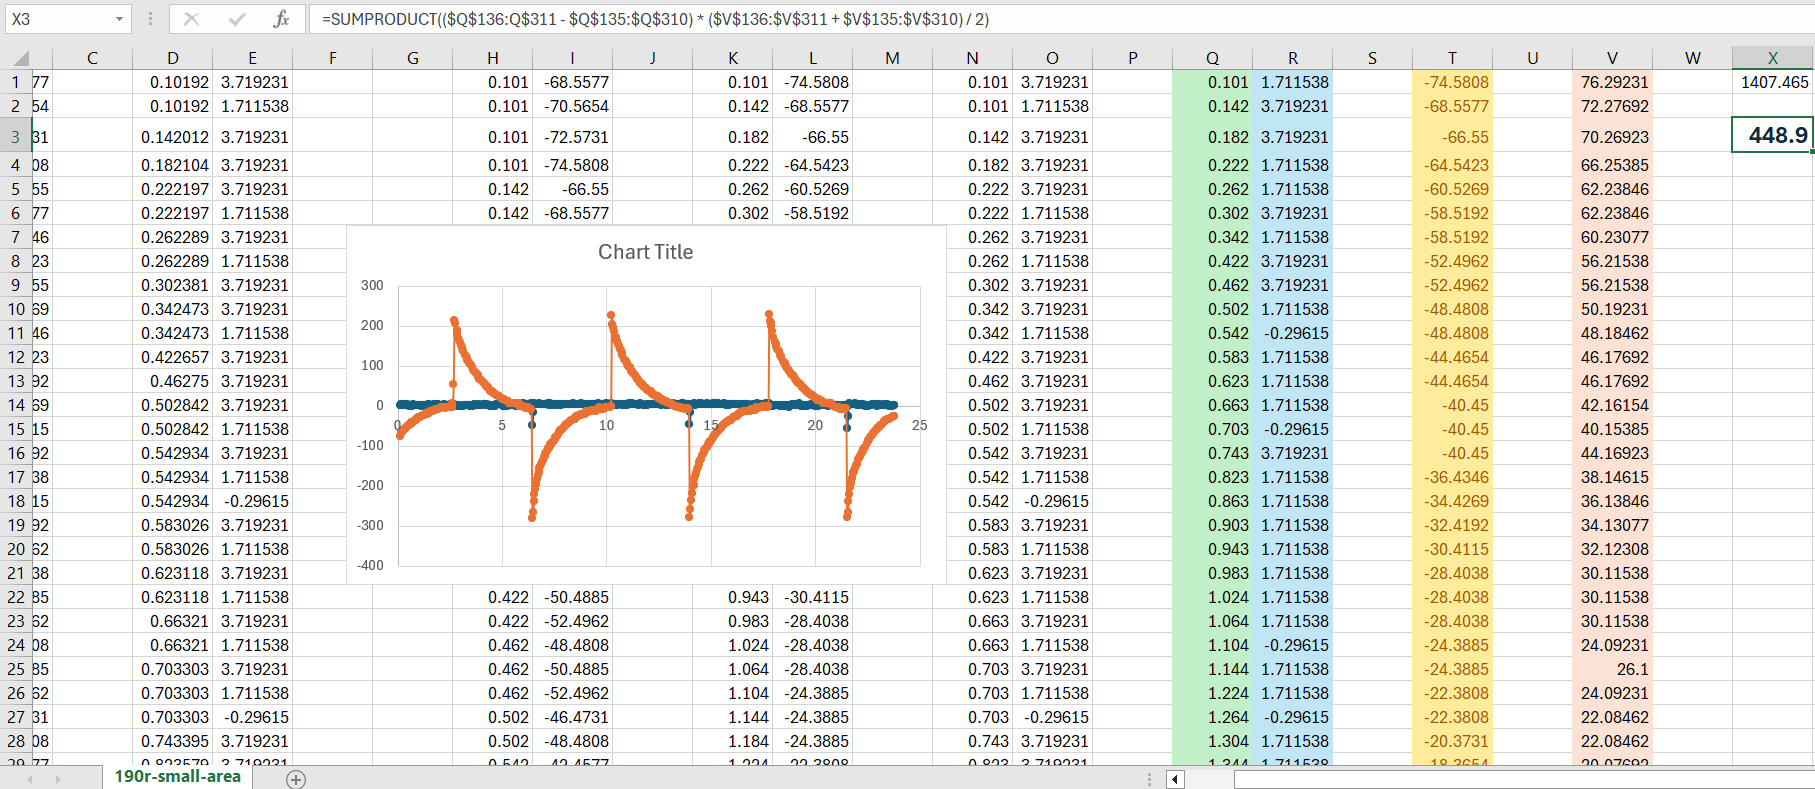
\includegraphics[width=1\textwidth]{figures/excel3.png}
    \caption{Beispiel für einen Excel-Arbeitsbereich zur Berechnung der Fläche zwischen zwei Kurven, wo Q ist die gemeinsame X-Koordinate, R ist die entsprechende Y-Koordinate für das blaue Diagramm, und T ist für das gelbe Diagramm. V-Differenz zwischen T und R. X3-Ergebnis}
    \label{img:excel_example}
\end{figure}

\subsection{Fehlerdiskussion}
\begin{enumerate}
    \item Integrierung das gesamte Diagramm:   
Zu Beginn wurde der gesamte Graph integriert und nicht nur eine Periode. Diese Ungenauigkeit führte zu weniger aussagekräftigen Daten, denn es besteht eine Abhängigkeit davon, in welcher Phase der Graph, der in das Bild fällt, beginnt.
    \item Auswahl unterschiedlicher Auflösungen für dasselbe Diagramm und für verschiedene Farben: 
    Bei der Wahl der idealen Auflösung wurde darauf geachtet, wie genau das Diagramm aussieht. Für unterschiedliche Kurven war ein bestimmtes Intervall besser geeignet (Abb. 4-5)  Aber ein solcher Unterschied in den Daten bedeutete, dass eine Farbe Informationen über 2000 verschiedene Punkte enthalten konnte und eine andere über 500. Der Vergleich solcher Daten läuft auf eine kleinere Zahl hinaus, sodass es keinen Sinn machte, hohe und niedrige Auflösungen zu haben. 

    Die Lösung bestand also darin, die optimale Anzahl für beide Farben zu finden
\end{enumerate}

\begin{figure}[ht]
    \centering
    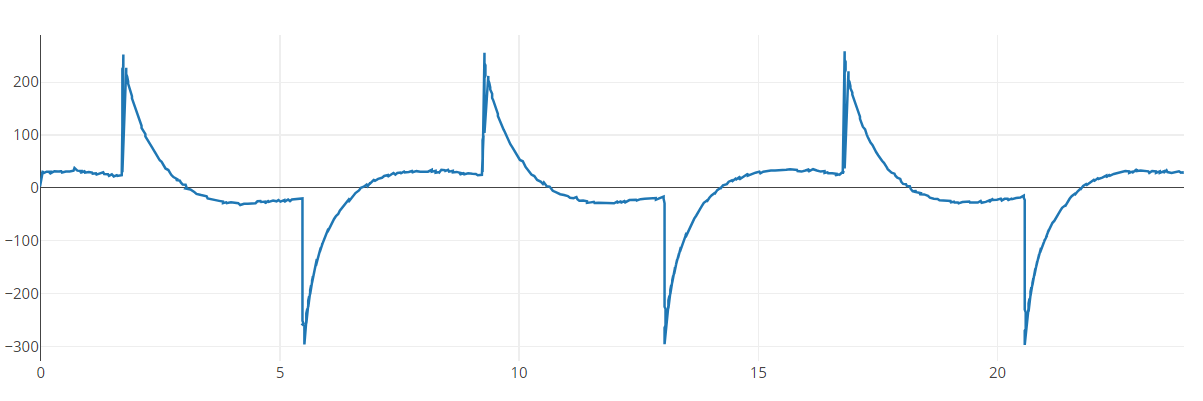
\includegraphics[width=\textwidth]{figures/1x-68kPf.png}
    \caption{Beispiel eines Diagramms mit Delta X = 1 (für einen 190 kΩ-Widerstand mit einem 68 000 pF-Kondensator)}
    \label{img:delta_x1}

    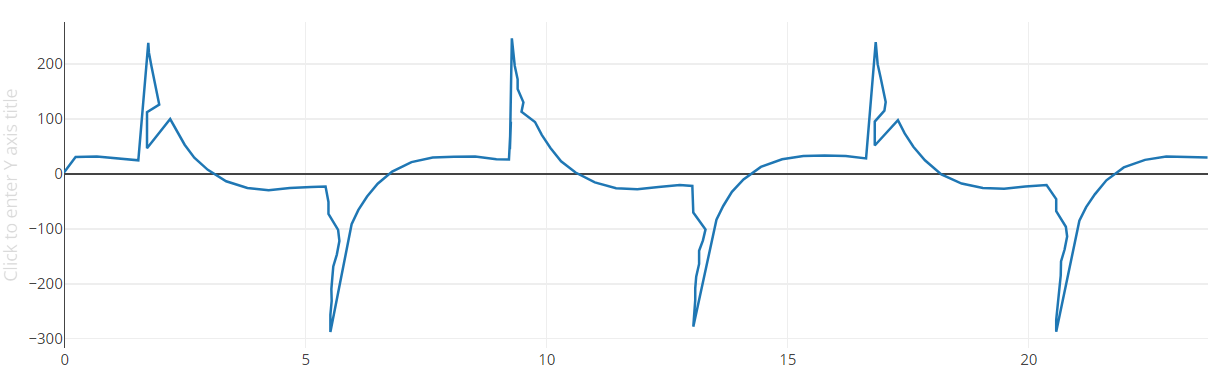
\includegraphics[width=\textwidth]{figures/10x-68kpF-190kOm.png}
    \caption{Beispiel eines Diagramms mit Delta X = 10 (für einen 190 kΩ-Widerstand mit einem 68 000 pF-Kondensator)}
    \label{img:delta_x10}
\end{figure}




%------------- Discussion -------------%
\section{Fazit}

Es konnte eine Veränderung der durchgelassenen Frequenzen festgestellt werden. Wie in Abbildungen \ref{fig:showcase_c68e3_r47} - \ref{fig:showcase_c33e0_r190} sichtbar, 

\begin{figure}[ht]
    \minipage{0.49\textwidth}
        \centering
        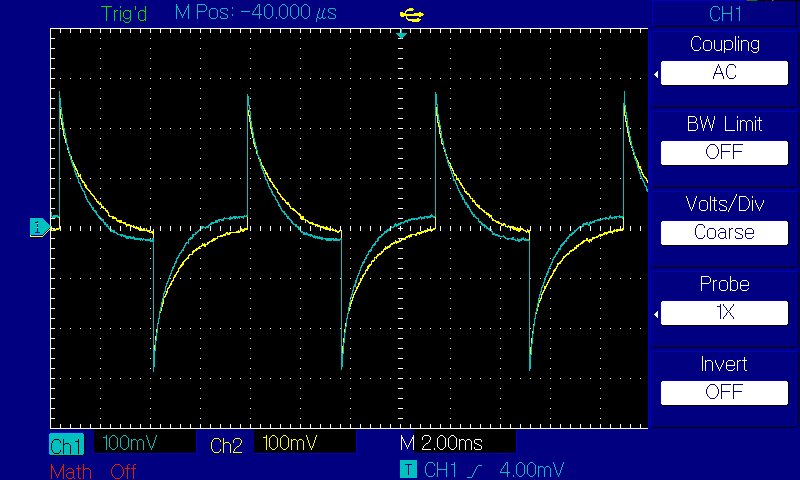
\includegraphics[width=\linewidth]{figures/results/resistor_47_Ohm/c68000pF.png}
        \caption{Screenshot vom Oszilloskop für Widerstand $R = 47k\Omega$ und Kapazität $C = 68nF$}
        \label{fig:showcase_c68e3_r47}
    \endminipage\hfill
    \minipage{0.49\textwidth}
        \centering
        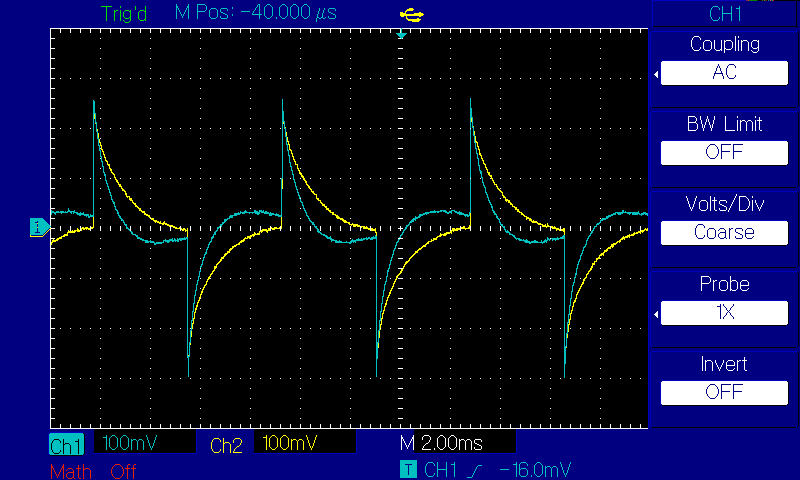
\includegraphics[width=\linewidth]{figures/results/resistor_190_Ohm/c68000pF.png}
        \caption{Widerstand $R = 190k\Omega$ und Kapazität $C = 68nF$}
        \label{fig:showcase_c68e3_r190}
    \endminipage\hfill
    \minipage{0.49\textwidth}
        \centering
        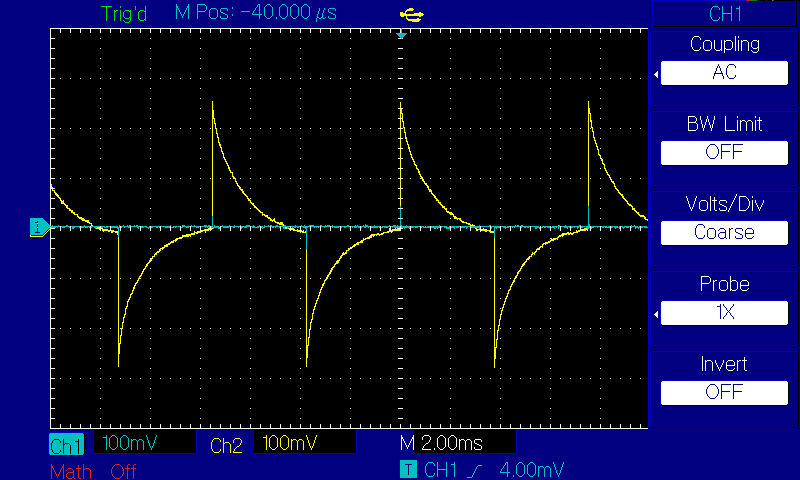
\includegraphics[width=\linewidth]{figures/results/resistor_47_Ohm/c33pF.png}
        \caption{Widerstand $R = 47k\Omega$ und Kapazität $C = 33pF$}
        \label{fig:showcase_c33e0_r47}
    \endminipage\hfill
    \minipage{0.49\textwidth}
        \centering
        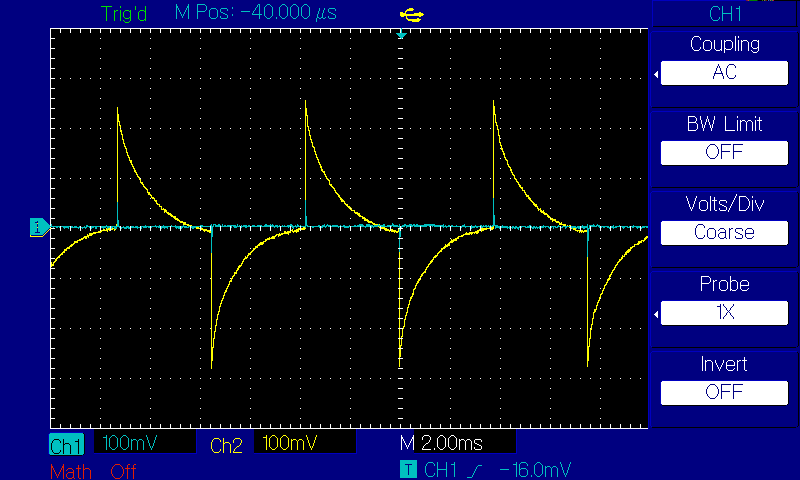
\includegraphics[width=\linewidth]{figures/results/resistor_190_Ohm/c33pF.png}
        \caption{Widerstand $R = 190k\Omega$ und Kapazität $C = 33pF$}
        \label{fig:showcase_c33e0_r190}
    \endminipage\hfill
\end{figure}

Die Integration des Graphen ist keine exakte Zahl, sondern eine grobe Annäherung. Viele verschiedene Faktoren, wie die Genauigkeit der Stichprobenpunkte, die Genauigkeit des Beginns und des Endes der Periode, die Größe des Intervalls zwischen x usw., könnten sich negativ auf die Genauigkeit des Ergebnisses auswirken.

Dennoch ist ein klarer Trend ersichtlich, dass je höher die Kapazität des Kondensators ist, desto mehr tiefere Frequenzen werden durchgelassen. Dies sieht man sehr klar an dem graphischen Unterschied zwischen Abbildungen \ref{fig:showcase_c33e0_r47} und \ref{img:showcase_c68e3_r47}, wie auch zwischen \ref{fig:showcase_c33e0_r190} und \ref{fig:showcase_c68e3_r190}. Mit einer Kapazität von $68nF$ wurde die Untersuchte Frequenz von $166.7Hz$ beinahe durchgelassen (Input- und Outputsignal der Volt-Kurven liegen sehr nahe beieinander), bei beiden Widerständen, auch wenn beim grösseren weniger. 

Dieselbe Frequenz wurde grösstenteils gefiltert mit einem Kondensator von $33pF$
Auch bei der numerischen Auswertung der Daten (Tabelle \ref{tab:integrals} ist dieser Trend sichtbar, wenn auch weniger offensichtlich. Dort scheinen die Werte für $190\Omega$ sehr nahe beieinander. Dies könnte durchaus von einem Rechenfehler herbeigeführt worden sein, da die Graphen sich deutlich unterscheiden.

Man kann auch sehen, dass die Graphen mit der Änderung des Kondensators bei niedrigem Widerstand viel mehr abweichen als bei hohem Widerstand (252,2 bei 47,3 und nur 86 bei 190 - Daten aus Tabelle 2).

Die genaue Grenze konnte jedoch nicht herausgelesen werden, wie auch die Art des Zusammenhangs zwischen Widerstand, Kapazität und Frequenz. Dazu wären mehr Messungen zu unterschiedlichen Widerständen nötig gewesen, aber schussendlich ist es an der numerischen Auswertung gescheitert. Da keinen Datenpunkte vom Oszilloskop, sondern nur Bilder extrahiert werden konnten, wurde die Auswertung stark erschwert und konnte nur für 4 Werte ausgeführt werden. Auch diese haben nur zweifelhafte Aussagekraft.
Qualitativ wurden jedoch alle Erwartungen erfüllt.

\newpage

\section{Bibliografie}
\printbibliography{} % Automatisch generierte Referenzen

\section{Anhang}

\emph{
    Alle Bilder, Tabellen sowie die Latex-Sourcen für diese Arbeit können unter
    \href{https://github.com/lrshsl/data/}{https://github.com/lrshsl/data/} im Ordner \emph{01 Audiofilter Hanna Lars} gefunden werden.
}

\newpage
\subsection{Werte für $R = 47k\Omega$}

\begin{figure}[!h]
    \minipage{0.48\textwidth}
        \centering
        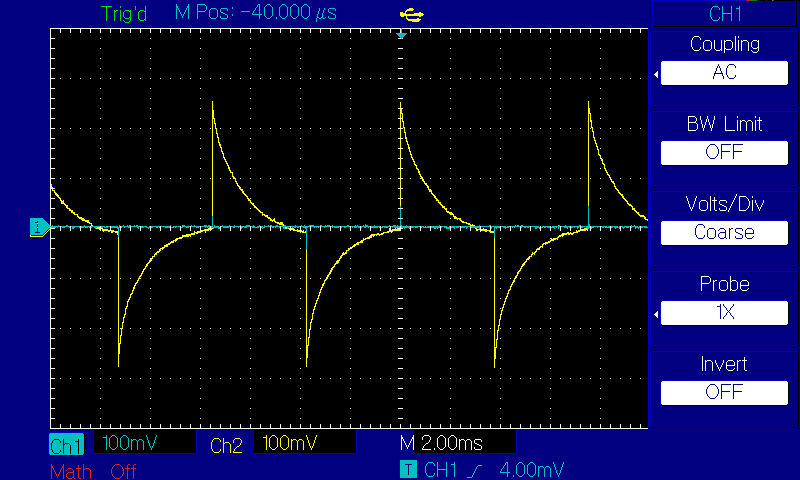
\includegraphics[width=\linewidth]{figures/results/resistor_47_Ohm/c33pF.png}
        \caption{Screenshot vom Oszilloskop für $C = 33pF$, Widerstand $R = 47k\Omega$}
        \label{img:c33e0_r47}
    \endminipage\hfill
    \minipage{0.48\textwidth}
        \centering
        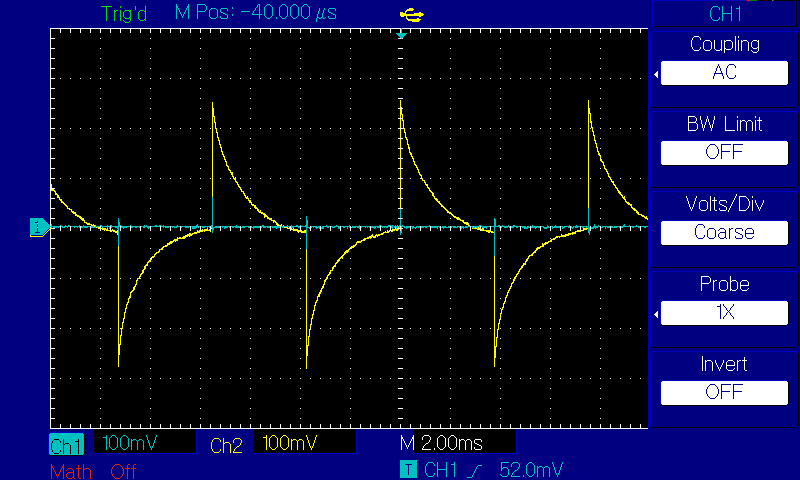
\includegraphics[width=\linewidth]{figures/results/resistor_47_Ohm/c68pF.png}
        \caption{$C = 68 pF$, $R = 47 k\Omega$}
        \label{img:c68e0_r47}
    \endminipage\hfill \\
    \minipage{0.48\textwidth}
        \centering
        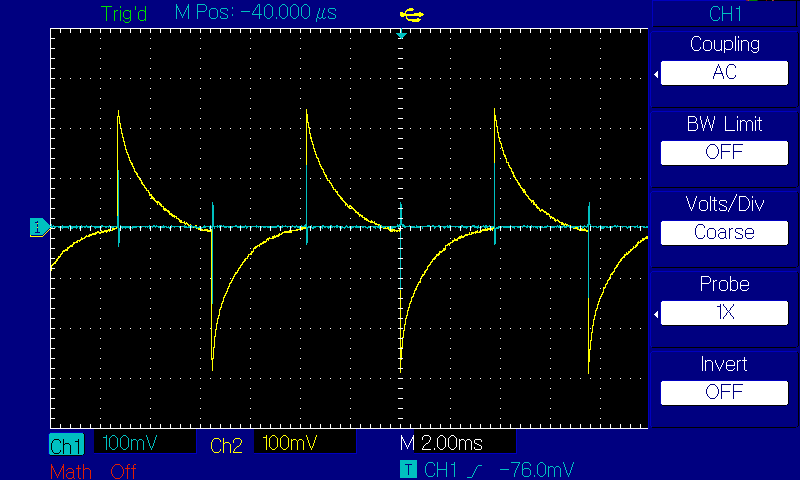
\includegraphics[width=\linewidth]{figures/results/resistor_47_Ohm/c330pF.png}
        \caption{$C = 330 pF$, $R = 47 k\Omega$}
        \label{img:c33e1_r47}
    \endminipage\hfill
    \minipage{0.48\textwidth}
        \centering
        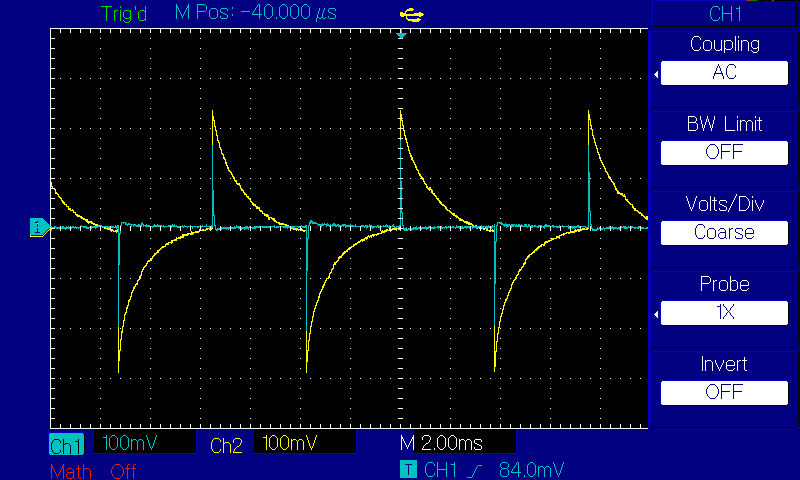
\includegraphics[width=\linewidth]{figures/results/resistor_47_Ohm/c680pF.png}
        \caption{$C = 680 pF$, $R = 47 k\Omega$}
        \label{img:c68e1_r47}
    \endminipage\hfill
\end{figure}
\begin{figure}[!h]
    \minipage{0.48\textwidth}
        \centering
        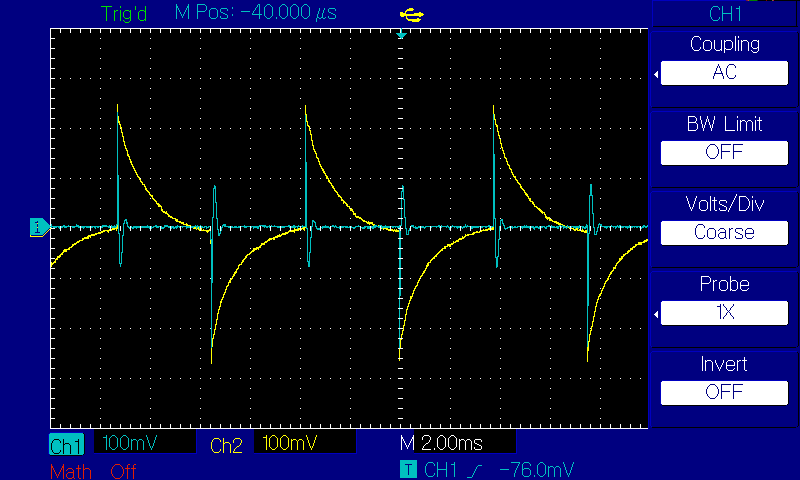
\includegraphics[width=\linewidth]{figures/results/resistor_47_Ohm/c3300pF.png}
        \caption{$C = 3300 pF$, $R = 47 k\Omega$}
        \label{img:c33e2_r47}
    \endminipage\hfill
    \minipage{0.48\textwidth}
        \centering
        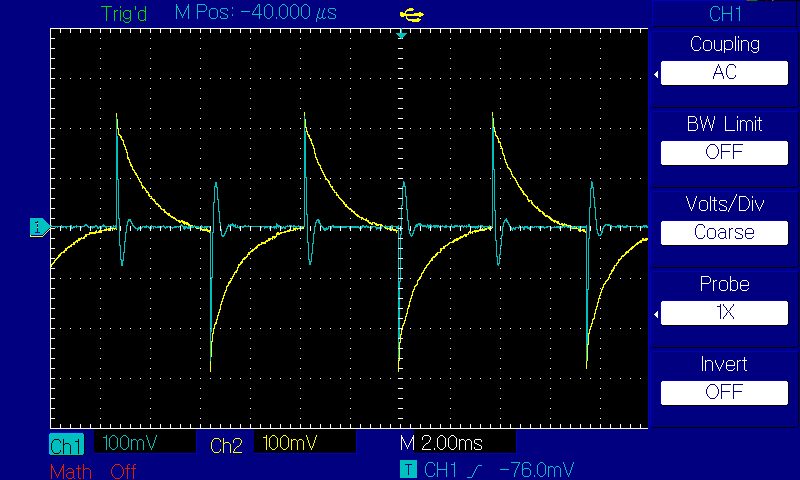
\includegraphics[width=\linewidth]{figures/results/resistor_47_Ohm/c6800pF.png}
        \caption{$C = 6800 pF$, $R = 47 k\Omega$}
        \label{img:c68e2_r47}
    \endminipage\hfill \\
    \minipage{0.48\textwidth}
        \centering
        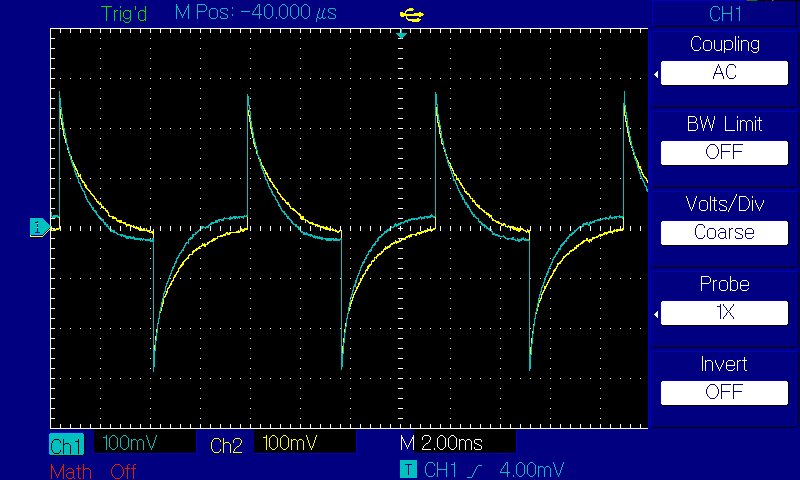
\includegraphics[width=\linewidth]{figures/results/resistor_47_Ohm/c68000pF.png}
        \caption{$C = 68000 pF$, $R = 47 k\Omega$}
        \label{img:c68e3_r47}
    \endminipage\hfill
\end{figure}

\newpage
\subsection{Werte für $R = 190k\Omega$}

\begin{figure}[!h]
    \minipage{0.48\textwidth}
        \centering
        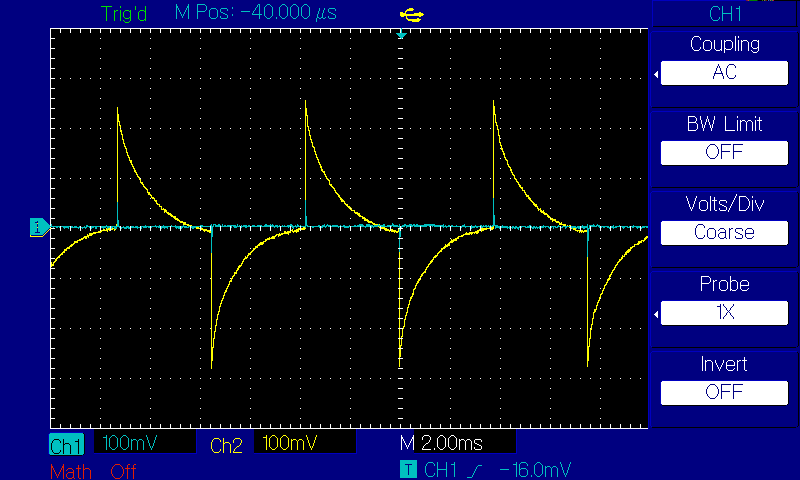
\includegraphics[width=\linewidth]{figures/results/resistor_190_Ohm/c33pF.png}
        \caption{Screenshot vom Oszilloskop für $C = 33pF$, Widerstand $R = 190k\Omega$}
        \label{img:c33e0_r190}
    \endminipage\hfill
    \minipage{0.48\textwidth}
        \centering
        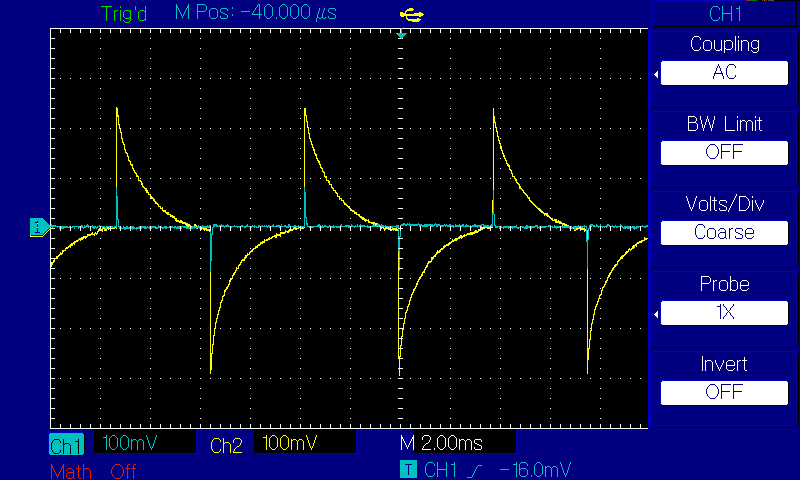
\includegraphics[width=\linewidth]{figures/results/resistor_190_Ohm/c68pF.png}
        \caption{$C = 68 pF$, $R = 190 k\Omega$}
        \label{img:c68e0_r190}
    \endminipage\hfill \\
    \minipage{0.48\textwidth}
        \centering
        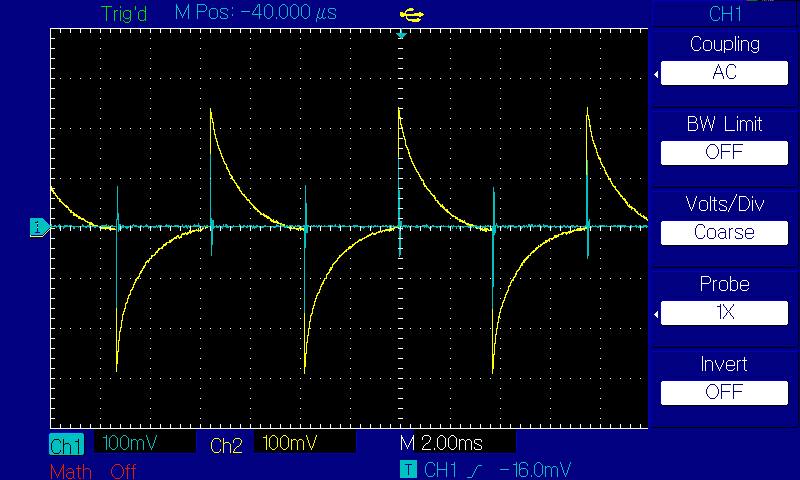
\includegraphics[width=\linewidth]{figures/results/resistor_190_Ohm/c330pF.png}
        \caption{$C = 330 pF$, $R = 190 k\Omega$}
        \label{img:c33e1_r190}
    \endminipage\hfill
    \minipage{0.48\textwidth}
        \centering
        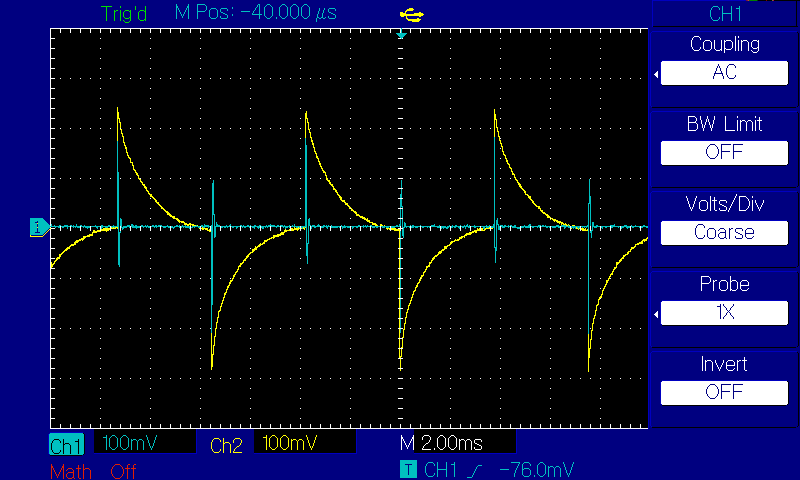
\includegraphics[width=\linewidth]{figures/results/resistor_190_Ohm/c680pF.png}
        \caption{$C = 330 pF$, $R = 190 k\Omega$}
        \label{img:c68e1_r190}
    \endminipage\hfill
\end{figure}
\begin{figure}[!h]
    \minipage{0.48\textwidth}
        \centering
        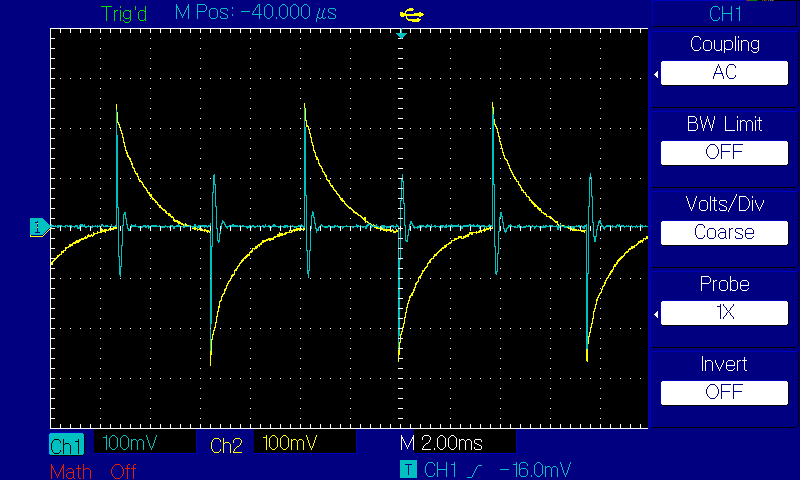
\includegraphics[width=\linewidth]{figures/results/resistor_190_Ohm/c3300pF.png}
        \caption{$C = 3300 pF$, $R = 190 k\Omega$}
        \label{img:c33e2_r190}
    \endminipage\hfill
    \minipage{0.48\textwidth}
        \centering
        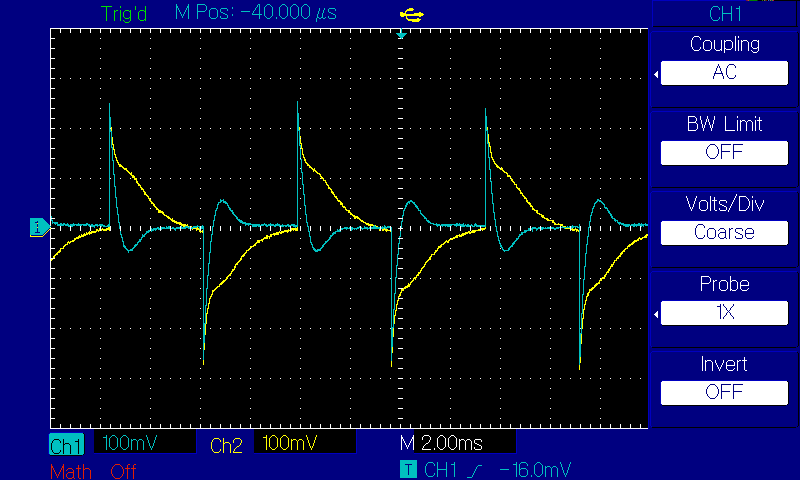
\includegraphics[width=\linewidth]{figures/results/resistor_190_Ohm/c6800pF.png}
        \caption{$C = 6800 pF$, $R = 190 k\Omega$}
        \label{img:c68e2_r190}
    \endminipage\hfill \\
    \minipage{0.48\textwidth}
        \centering
        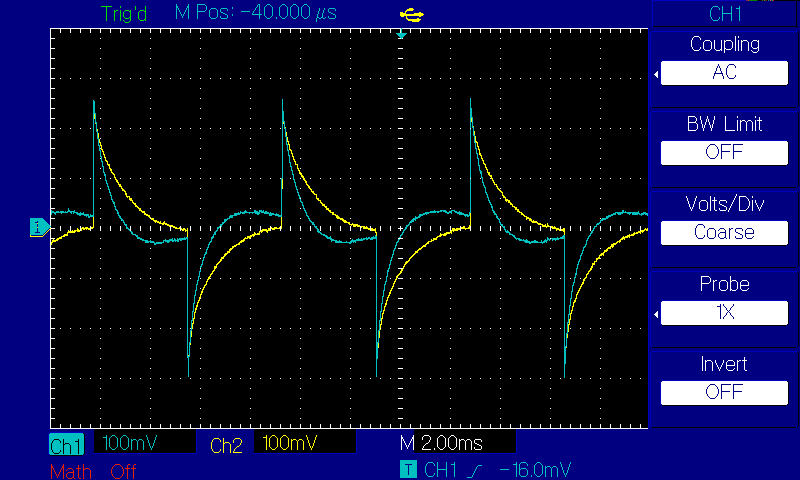
\includegraphics[width=\linewidth]{figures/results/resistor_190_Ohm/c68000pF.png}
        \caption{$C = 68000 pF$, $R = 190 k\Omega$}
        \label{img:c68e3_r190}
    \endminipage\hfill
\end{figure}

\end{document}
